\documentclass[12pt]{article}

\usepackage[letterpaper,top=2cm,bottom=2cm,left=3cm,right=3cm,marginparwidth=1.75cm]{geometry}

\usepackage{amsmath, amsfonts, amssymb}
\usepackage{graphicx}
\usepackage{algorithm}
\usepackage[noend]{algpseudocode}
\usepackage{amsthm}
\usepackage{bm}
\usepackage{cases}
\usepackage{caption}
\usepackage{hyperref}
\usepackage{multirow}
\usepackage{bbm}
\usepackage{booktabs}
\usepackage{siunitx}
\newcolumntype{d}{S[table-format=3.2]}


\DeclareMathOperator*{\argmin}{argmin}


\usepackage{setspace}
 \doublespacing 

\usepackage{soul}
\usepackage{xcolor}
\def\bwr#1{{\color{violet}\textbf{BWR:[#1]}}}

\newcommand{\pkg}[1]{{\normalfont\fontseries{b}\selectfont #1}}
\let\proglang=\textsf \let\code=\texttt


\usepackage{natbib}
\bibliographystyle{apalike}

\title{Bayesian Modeling of Overdispersed Longitudinal Zero-Inflated Binomial Data}
\author{Benjamin W. Rogers and Robert E. Weiss}

\begin{document}

\newcommand{\del}[2]{\frac{\partial {#1} }{\partial {#2}} }
\newcommand{\dby}[2]{\frac{d {#1} }{d {#2}} }
\newcommand{\sbar}{\overline{s}}
\newtheorem{proposition}{Proposition}

\theoremstyle{remark}
\newtheorem*{remark}{Remark}

\maketitle

\begin{abstract}
 We develop a class of longitudinal overdispersed zero-inflated binomial (LOZIB) models for use in overdispersed repeated measures count data with a large number of zero observations. These LOZIB models extend previous zero-inflated regression models by incorporating observation-level random effects (OLRE), which allow more flexibility to account for excess variability as well as correlation over time through the specification of within-individual covariance models. We present an analysis of the number of days of heavy drinking in a study of screening, brief intervention, and referral to treatment (SBIRT) using LOZIB models with 10 different covariance models, and show all of them to outperform previously developed subject level random intercept zero-inflated models. These models are implemented in a Bayesian framework using Stan software.
\end{abstract}

\section{Introduction}
\label{s:intro}


It is common for count data to have excess zeros relative to standard distributions, known as zero-inflation. This often happens in settings where zeros have a special meaning and can be created by a process separate from that which produces the counts. For example, we consider the number of days of heavy drinking in a population of high risk individuals. We observe a large number of zeros because not all subjects engage in heavy drinking. Thus, zero counts can come from two different processes -- a person may engage in no heavy drinking because this is not an activity they engage in, or a person may occasionally drink heavily, but happen to not do so during the observed time interval. We call these structural and random zeros, respectively.

Our interest is in estimating the effect of a Screening, Brief Intervention and Referral to Treatment (SBIRT) intervention to reduce alcohol and drug use in a population of substance users seeking mental health treatment \citep{karno2021effect}. SBIRT has received attention recently as a treatment approach for substance use disorder (SUD) \citep{saitz2014screening, glass2015specialty, barata2017effectiveness, tetrault2020computerized}. We analyze data consisting of 718 patients aged 18 and older randomized into either SBIRT or standard of care treatment groups. To be eligible for the study, subjects had to have a mental health disorder and report use of cannabis, stimulants or one or more days of heavy drinking ($\geq 5$ drinks for men, $\geq 4$ drinks for women). Subjects were brought in for a baseline visit, and followed up with at 3, 6, and 12 months -- at each visit, a number of variables were recorded including the number of days out of the previous 90 that each subject engaged in heavy alcohol use. As subjects were eligible for the study for using any of a variety of substances, a large number of zero counts were observed in days of heavy drinking (Figure \ref{fig:inflation}).

\begin{figure}[ht]
	\centering
	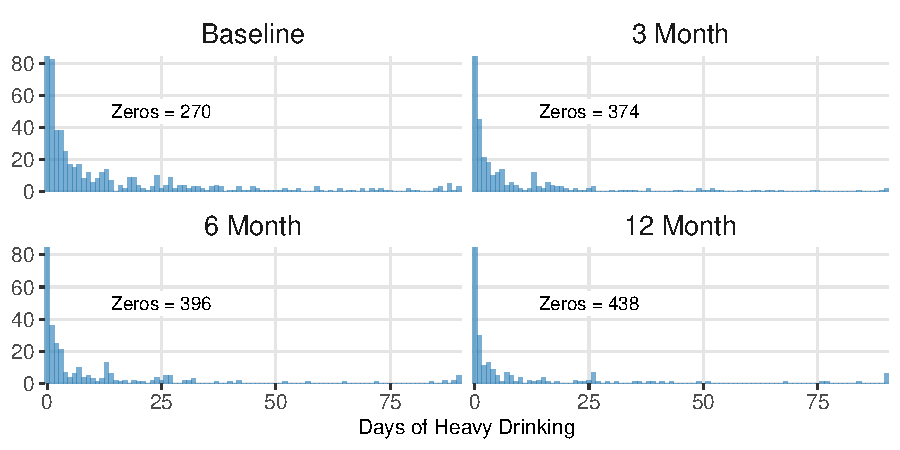
\includegraphics[scale=1]{figures/inflation_heavy_plot.pdf}
	\caption{Self-reported days out of the previous 90 in which subjects engaged in heavy drinking at baseline and 3, 6 and 12 month follow-ups. The distribution of responses is both zero-inflated and over-dispersed.}
	\label{fig:inflation}
\end{figure}

A standard approach to modeling such data are a class of mixture models known as zero-inflated models \citep{cohen1966note, johnson2005univariate, ridout1998models}, which are comprised of two parts -- a zero model and a count model. The zero model uses a Bernoulli distribution to model a latent binary variable representing whether or not an observation is a structural zero. In modeling heavy drinking, this binary variable represents whether or not a subject may engage in heavy drinking. Conditional on not being a structural zero, the count model uses a count distribution, such as a binomial, negative binomial or Poisson distribution, to model the observations that are not structural zeros. 

Covariates can be controlled for using generalized linear regression models in both the zero and count models \citep{mullahy1986specification, lambert1992zero, heilbron1994zero}. For longitudinal repeated measures data, \cite{hall2000zero} developed zero-inflated binomial models using subject-level random intercepts in the count model to account for within-individual correlation over time. \cite{yau2001zero} extend Hall's model by including independent subject-level random intercepts in both the zero and count models. \cite{lee2006multi} include include independent cluster and subject-level random effects in both parts of the zero-inflated model. \cite{min2005random} make the argument that there is likely correlation between an individual's zero and count model means, which they model using a bivariate normal distribution for the zero and count model random intercepts. In addition, \cite{buu2012statistical} developed a version of Min and Agresti's model which includes non-linear time trends in both the zero and count regression models. Other authors have extended the zero-inflated Poisson model for multivariate zero-inflated outcomes \cite{wu2023multivariate, liu2015type}

We develop models in a Bayesian framework, which allows for numerous advantages including the ability to incorporate prior information and to make inference on possibly complex functions of model parameters \citep{gelman2013bayesian}. Frequentist methods to produce inference on covariate-adjusted marginal means have been developed for zero-inflated models \citep{albert2014estimating, preisser2016marginalized}. Using a Bayesian approach, posterior distributions for such inferences are straightforward to compute. Several authors have proposed Bayesian approaches to zero-inflated models.  \cite{rodrigues2003bayesian} and \cite{ghosh2006bayesian} present Bayesian zero-inflated models, using a latent variable data augmentation approach to aid in posterior sampling. \cite{wen2024bayesian} present another data augmentation approach for zero-inflated models using a mixture of P\'{o}lya-Gamma distributions. \cite{neelon2010bayesian} give a Bayesian adaptation of Min and Agresti's model, with correlated subject-level random intercepts \citep{spiegelhalter1998bayesian, cooper2007predicting}.

Zero-inflation is one type of overdispersion - when the observed variation is larger than what is expected from a given model. However after accounting for zero-inflation, there may be other sources of overdispersion in the count model. When this occurs one may consider using a different distribution. For example the negative binomial distribution models overdispersion compared to a Poisson \citep{gardner1995regression}. \cite{hinde1998overdispersion} introduce a score test for deciding between a zero inflated Poisson (ZIP) and zero-inflated negative binomial (ZINB) distribution. For overdispersed binomial data, one may use a beta-binomial distribution \cite{hu2018zero, wen2024bayesian}. An alternative approach for overdispersion is to include observational level random effects (OLRE)  \cite{harrison2014using}. Here we explore the use of OLRE in zero-inflated binomial models as they also provide a straightforward framework through which to model longitudinal correlation.

In repeated measures studies, observations on the same individual will generally be positively correlated. Random intercept models allow for this, but do so rather rigidly. For example, it is also reasonable to expect this correlation to differ between different pairs of measurements, decreasing as time between observations increases, a quality which cannot modeled with random intercepts. Additionally, it is common to observe heterogeneity over time, as variability often increases with time since intervention, which is also not allowed for in random intercept models.

It has been shown that choice of covariance models in longitudinal data impacts inference \citep{lange1989effect, wolfinger1996heterogeneous}. Models should be complex enough to reflect the data generating process, but modeling unnecessary parameters can result in a loss of power. The random intercept model has been shown to be insufficient in many settings compared to more flexible covariance models \citep{barr2013random, kwok2007impact}.  We explore the use of covariance models of varying complexity, ranging from the random intercept (simplest) to the unstructured (most flexible), in zero-inflated binomial models, finding that the more complex covariance structures vastly improve model performance.

We introduce a class of longitudinal overdispersed zero-inflated binomial (LOZIB) regression models. These models extend previous zero-inflated models by using observation-level random effects (OLRE) in the count model to account for additional variation and correlation over time.  Within-individual correlation over time is modeled through correlation between an individual's OLRE. We consider various specifications of covariance models and compare against previously used random intercept models, finding the loZIB models to fit the data considerably better.

\section{Model}
\label{s:model}

Let $Y_{ij}$ be a zero inflated count response for subject $i=1,\dots,N$ at visit $j=1, \dots, J$ where $N$ is the total number of subjects, $J$ is the number of visits per subject and $y_{ij}$ is the observed data. Then we consider a two part model
\begin{align}
	P(Y_{ij} = 0 | \pi_{ij}, \theta_{ij}) &= (1 - \pi_{ij}) + \pi_{ij} f(0 | \theta_{ij}), \label{eq:zip1} \\
	P(Y_{ij} = y_{ij} | \pi_{ij}, \theta_{ij}) &= \pi_{ij} f(y_{ij}| \theta_{ij}), \; y_{ij}=1, \dots, \infty \label{eq:zip2}
\end{align}
where $1-\pi_{ij}$ is the probability of being a structural zero for subject $i$ at time $j$, and $f(k| \theta_{ij})$ is the probability density function for some discrete distribution with parameter $\theta_{ij}$, such as the binomial, negative binomial or Poisson. This is the form of the standard zero-inflated count model. Equation \eqref{eq:zip1} follows from the fact that zeros can either be structural, with probability $1-\pi_{ij}$, or random, with probability $\pi_{ij} f(0 | \theta_{ij})$. Similarly, Equation \eqref{eq:zip2} follows because to observe a positive count, that observation must not be a structural zero, which happens with probability $\pi_{ij}$, and is then modeled with the count distribution $f(y_{ij}| \theta_{ij})$.

In the SBIRT application, $\pi_{ij}$ is the probability that person $i$ is a heavy drinker at visit $j$. If a subject is a heavy drinker, we model the number of days out of 90 in which they drink heavily with distribution function $f(y_{ij}| \theta_{ij})$ which follows a binomial($90, \theta_{ij}$) distribution where $\theta_{ij}$ is the probability subject $i$ drinks heavily on any individual day during the 90 days observed at visit $j$. 

\subsection{Random Intercept Model} \label{sec: rimodel}
The two parameters $\pi_{ij}$ and $\theta_{ij}$ can be modeled using mixed effects regression. For some appropriate link functions $g_{1}(\cdot)$ and $g_{2}(\cdot)$
\begin{align}
	g_{1}(\pi_{ij}) &= \bm{X}_{1ij} \bm{\beta_{1}} + \gamma_{1i} \label{eq:linearzerori}\\ 
	g_{2}( \theta_{ij}) &= \bm{X}_{2ij} \bm{\beta_{2}} + \gamma_{2i}, \label{eq:linearcountri}
\end{align}
where $\bm{X}_{1ij}$ and $\bm{X}_{2ij}$ represent fixed effect covariate vectors of lengths $K_{1}$ and $K_{2}$ for subject $i$ at time $j$ with corresponding unknown coefficient vectors $\bm{\beta_{1}}$ and $\bm{\beta_{2}}$, and each subject $i$ has random intercept $\gamma_{1i}$ for the zero model and $\gamma_{2i}$ for the count model. Within-individual correlation over time is modeled through $\gamma_{1i}$ and $\gamma_{2i}$. Let $g_{1}(\pi_{ij}) = \text{logit}(\pi_{ij}) = \log(\pi_{ij})/(1- \log(\pi_{ij}))$, the logit link function, as is standard in logistic regression, while $g_{2}( \theta_{ij})$ is some appropriate link function for the count model. In the SBIRT analysis, we also choose $g_{2}( \cdot)$ to be the logit function for the binomial distribution. For other distributions, one may wish to use a different link function, such as the log function for the Poisson distribution.

The random intercepts are assumed to follow a bivariate normal distribution,
\begin{equation}
	\mathbf{\gamma}_{i} = 
	\begin{pmatrix}
		\gamma_{1i} \\
		\gamma_{2i}
	\end{pmatrix}
	\sim
	\text{N}_2 \left(
	\mathbf{0}
	, \mathbf{\Sigma}
	\right),
	\label{eq:RIdistribution}
\end{equation}
where the off diagonal element $\sigma_{12}$ of the $2 \times 2$ covariance matrix $\mathbf{\Sigma}$ models the correlation between an individual's zero model and count model random intercepts. Equations \eqref{eq:zip1} - \eqref{eq:RIdistribution} define the zero-inflated model proposed by \cite{min2005random}. One can set a prior distribution on $\mathbf{\Sigma}$ to take a Bayesian approach to Min and Agresti's model. \cite{neelon2010bayesian} take a Bayesian approach by setting a marginal density for $\gamma_{1i}$ and a conditional density for $\gamma_{2i}|\gamma_{1i}$ \citep{spiegelhalter1998bayesian, cooper2007predicting} on the random effects
\begin{align}
	\gamma_{1i} &\sim \text{N}(0, \sigma_{1}^{2}) \label{eq:zero_ri_dist}\\
	 \gamma_{2i}|\gamma_{1i} &\sim \text{N}(\psi \gamma_{1i}, \sigma_{2}^{2}), \label{eq:count_ri_dist}
\end{align}
and with some diffuse hyperpriors on $\sigma_{1}^2$, $\sigma_{2}^{2}$ and $\psi$.

\subsection{Longitudinal Overdispersed Zero-Inflated Binomial Model (LOZIB)}

We propose a class of longitudinal overdispersed zero-inflated binomial models (LOZIB) which extend the model of the previous section by introducing observation-level random effects into the count model. Thus, equation \eqref{eq:linearcountri} become
\begin{align}
	g_{2}( \theta_{ij}) &= \bm{X}_{2ij} \bm{\beta_{2}} + \psi \gamma_{1i} + \gamma_{2ij} \label{eq:linearcountOLRE}
\end{align}
where each subject $i$ has random effect $\gamma_{1i}$ for the zero model and a vector of random effects $\bm{\gamma_{2i}}= (\gamma_{2i1}, \gamma_{2i2}, \dots, \gamma_{2iJ})' $ for the count model while equation \eqref{eq:linearzerori} for the probability of a zero remains the same.  We model correlation between the count and zero models through the additive term $\psi \gamma_{1i}$ and center the count model random effects $\bm{\gamma}_{2i}$ around zero
\begin{equation}
	\bm{\gamma}_{2} \sim \text{N}_{J} (\bm{0}, \bm{\Sigma}_{2}),\label{eq:count_olre_dist}
\end{equation}
where covariance matrix $\bm{\Sigma}_{2}$ models within-individual variation and correlation over time and $\bm{0}$ denotes a vector of zeros of length $J$. This class of models has numerous benefits over the random intercept including additional flexiblity for temporal correlation, and heterogeneity. We do not include OLRE in the zero model as this would be overparamaterized given that there is relatively little information for modeling an unobserved binary variable.

\subsection{Covariance Models}
The LOZIB models provide a convenient framework for modeling within-individual correlation over time through specification of $\bm{\Sigma}_{2}$, the count model random effects covariance matrix. Let 
\begin{equation}
	\bm{\Sigma}_{2} = \text{diag}(\bm{\sigma}_{2}) \Omega \text{diag}(\bm{\sigma}_{2}),
	\label{eq:CovDeconstruct}
\end{equation}
where $\text{diag}(\bm{\sigma}_{2})$ is a diagonal matrix with diagonal entries given by the vector of standard deviations $\bm{\sigma}_{2} = (\sigma_{21}, \dots, \sigma_{2J})'$, and $\Omega$ is a $J \times J$ matrix of correlations. This is a heteroskedastic model, as the standard deviation is allowed to vary over time. One can also consider a homoskedastic, or constant variance, model by assuming the standard deviation to be constant over time such that $\sigma_{2j} \equiv \sigma_{2}$ for all $j=1, \dots, J$. In the homoskedastic case, the scalar $\sigma_{2}$ replaces the $\text{diag}(\bm{\sigma}_{2})$ term in equation \eqref{eq:CovDeconstruct}. Within individual correlation over time is modeled through $\Omega$, which can be parameterized using an appropriate correlation model \citep{liechty2004bayesian, weiss2005modeling}. We present three possible correlation models, each of which may be paired with constant or non-constant variance over time.

\paragraph{Independence:}
The independence (IND) model is the simplest of the covariance models presented in this paper. It assumes count model random effects within an individual are independent over time. The correlation matrix $\bm{\Omega}_{IND} = \bm{I}_{J}$ where $\bm{I}_{J}$ is the $J \times J$ identity matrix. The IND model assumes no correlation between an individual's random effects across time.

\paragraph{Compound Symmetry:}
The compound symmetry (CS) model is a one parameter model which assumes equal correlation, $\rho$, between any two observations from the same individual. Thus, Corr$(\gamma_{2ij}, \gamma_{2ik}) = \rho$ for all $j \neq k$. While this is an improvement over the IND model, in that it allows for correlation between observations mad on the same individual, one would typically expect observations made closer in time to have higher correlation, which the CS model does not allow for. 

\paragraph{Autoregressive:}
The autoregressive correlation model (AR) is a one parameter model which assumes a constant correlation between any two \textit{adjacent} time points. For the SBIRT data, with $J=4$ visits, the correlation matrix of $\bm{\gamma}_{2i}$ is
\begin{equation*}
	\text{Corr}(\bm{\gamma_{2i}}) = \bm{\Omega}_{\text{AR}}(\rho) =
	\begin{pmatrix}
		1 & \rho & \rho^{2} & \rho^{3} \\
		\rho & 1 & \rho & \rho^{2}\\
		\rho^{2} & \rho & 1 & \rho \\
		\rho^{3} & \rho^{2} & \rho & 1
	\end{pmatrix}.
\end{equation*}
As observations get more distant in time, the correlation between the corresponding random effects decays, which one would expect in most longitudinal data. An appeal of using the autoregressive correlation model is that no matter how large $J$ is, only one parameter $\rho$ needs to be estimated. 
\paragraph{Antedependent:}
The antedependence model generalizes the AR model, with $J-1$ distinct correlations between consecutive observations. It is a good candidate covariance model for the SBIRT data where the spacing between consecutive time points differs over the course of the study. For the SBIRT setting with $J=4$ visits,
\begin{equation*}
	\bm{\Omega}_{\text{AD}}(\bm{\rho})= 
	\begin{pmatrix}
		1 & \rho_{1} & \rho_{1} \rho_{2} & \rho_{1} \rho_{2} \rho_{3}\\
		\rho_{1} & 1 & \rho_{2} & \rho_{2} \rho_{3}\\
		\rho_{1} \rho_{2} & \rho_{2} & 1 & \rho_{3} \\
		\rho_{1} \rho_{2} \rho_{3} & \rho_{2} \rho_{3} & \rho_{3} & 1
	\end{pmatrix}
\end{equation*}
where the lag 1 correlations are given by the elements of $\bm{\rho} = (\rho_{1}, \dots, \rho_{3})'$.

\paragraph{Unstructured:}
The unstructured correlation model (UN) is the most flexible correlation model and makes no assumptions about the correlations between random effects, however the number of correlation parameters to estimate grows as $J^2$, which can be costly in settings with many repeated measures. Possible priors for the UN correlation matrix include the LKJ prior \citep{lewandowski2009generating} and Wishart-based correlation distribution \citep{zhang2006sampling}.

\subsection{Markove Chain Monte Carlo}

The models as parameterized in the previous sections suffered from slow mixing. Here we present alternative parameterizations for each of the models for use in Bayesian sampling, which greatly improved posterior sampling performance.This consisted of sampling standardized random effects from standard normal distributions and then using these to construct random effects with the desired distributions.

For the RI model subject-level random effects, we model $Z_{1i}$, $Z_{2i} \sim \text{N}(0,1)$ distributions and then define appropriately scaled random effects $\gamma_{1i} = \sigma_{1}Z_{1i}$ and $\gamma_{2i}=\sigma_{2}Z_{2i}$. 

Similarly, for the LOZIB model observation-level random effects, model $Z_{1i}, Z_{2ij} \sim $N$(0,1)$. We take two different approaches to parameterizing the LOZIB models, one for the AD, AR, homoskedastic AD (ADcv) and homoskedastic AR models (ARcv), and a slightly different approach for the UN models.

The ADcv, AR and ARcv models are special cases of the more general heteroskedastic AD model. For the AD model, the observation-level random effects are parameterized
\begin{align}
	\gamma_{2i1} = \sigma_{21} Z_{2i1}
\end{align}
and for $j>1$,
\begin{align}
	\gamma_{2ij} = a_{j-1} \gamma_{2ij-1} + s_{2j} Z_{2ij}
\end{align}
where $a_{j-1} = \rho_{j-1} \frac{\sigma_{2j}}{\sigma_{2j-1}}$ and $s_{2j} = \sqrt{(1 - \rho_{j-1}^{2})}\sigma_{2j}$. When $\rho_{j-1} \equiv \rho$ for all $j>1$, we get the AR model. For both the AR and AD models, letting $\sigma_{2j} \equiv \sigma_{2}$ for all $j$, we get the homooskedastic or constant variance models (ADcv and ARcv).

Using the Cholesky factorization $\bm{\Omega}_{\text{UN}} = LL'$ with lower triangular matrix $L$, let
\begin{equation}
	\bm{\gamma}_{2i} = \text{diag}(\bm{\sigma}_{2}) L\; \bm{Z}_{i}
\end{equation}
where $\bm{Z}_{i} = (Z_{i1}, \dots, Z_{iJ})'$, and $\text{diag}(\bm{\sigma}_{2})$ is a diagonal matrix with $j$th diagonal entry $\sigma_{2j}$.

We fit all models in Stan \citep{gelman2015stan} with the \texttt{cmdstanr} package \citep{gabry2021cmdstanr} for R \citep{rsoftware}.


\subsection{Difference of Differences} \label{sec: DoD}

Fitting a zero-inflated model results in two sets of parameters, one for the zero model, and one for the count model. Researchers are often primarily interested the overall effect of a covariate on the overall outcome which requires combining the two parts of the model. The Bayesian approach allows straightforward inference on complex functions of parameters. In the SBIRT analysis, can calculate posterior distributions of mean days of heavy drinking for each treatment group at each time point, as well as differences in treatment effect between groups, combining both model parts rather than making inference on the zero and count models separately.

Our primary goal in the SBIRT analysis is to assess the effectiveness of the SBIRT intervention compared to the standard of care in reducing frequency of heavy drinking. Let $\mu_{jc}$ be the mean days of heavy drinking at time $j$ for treatment group $c=1,2$ for the control and treatment group respectively. Then the difference of differences (DoD) at visit $j$ is
\begin{align}
	\text{DoD}(\bm{\mu}_{j}) = (\mu_{12} - \mu_{02}) - (\mu_{j1}-\mu_{11}),
\end{align}
and can be understood as the difference in treatment effect between treatment groups at time $j$, where treatment effect is measured as the reduction in frequency of heavy drinking.

We quantify this with the difference of differences (DoD$(\bm{\mu}_{j})$), the difference in change from baseline at visit $j$ in expected number of days of heavy drinking between the SBIRT and control groups. We can calculate the DoDs separately for each of the two parts of the zero-inflated model in a similar fashion.

%Posterior inferences of DoDs
Calculating the posterior distributions of the various DoDs requires integrating out random effects, which we do using Monte Carlo methods. Let $\zeta^{(s)} = (\bm{\beta}_{1}^{(s)}, \bm{\beta}_{2}^{(s)}, \sigma_{1}^{(s)}, \bm{\Sigma_{2}}^{(s)})$ be posterior sample $s = 1, \dots, S$, where $S$ is the total number of posterior draws. For each $\zeta^{(s)}$, we drew 1,000 samples from random effects distributions \eqref{eq:zero_ri_dist} and \eqref{eq:count_olre_dist} and used these samples to integrate out the random effects to compute estimates of the marginal means of the zero and count models at each visit for each treatment group. From the zero and count model means, one can also compute the overall mean of the zero-inflated model, as well as the DoDs described in section \ref{sec: DoD}.


\subsection{Prior Distributions}

Priors were selected to be generally vague to let data dictate the inference. Elements of fixed effect vectors $\beta_{lk} \sim \text{N}(0, 10^2)$ for $l=1,2$, and $k=1,\dots, K_{l}$. The standard deviation parameters $\sigma_{1}$ and $\sigma_{2}$ for homoskedastic models (RI, AR, AD), and $\sigma_{2j}$ for the heteroskedastic models (AR, AD, UN) were given half-normal N$^+$($0$,$.5^2$) priors where N$^+$(a,b) is the Normal distribution with mean a and variance b restricted to the positive domain.

for the zero model random intercepts and count model random effects were given half-normal N$^+$($0$,$.5^2$) priors where N$^+$(a,b) is the Normal distribution with mean a and variance b restricted to the positive domain. The regression coefficient $\psi$ modeling the association between the zero and count models was given a N$^+$($0$,$1^2$) prior, as we expect a positive correlation between an individual's zero model and count model estimates. Correlation parameters $\rho$ for the AR models, and elements of $\bm{\rho}=(\rho_{1}, \rho_{2}, \rho_{3})$ in the AD models -- were assigned flat U($0$,$1$) priors, again reflecting the expected positive within-individual correlation. We set an LKJ correlation prior \citep{lewandowski2009generating} for the correlations of the UN covariance matrix , with shape parameter $\eta=1$ corresponding to a uniform distribution over all correlation matrices of order $J$.


\section{SBIRT Data Analysis}

\begin{enumerate}
	\item Model Fit
	\begin{enumerate}
		\item Make new plot of means and DoDs. Try to do the same with all substances, but maybe remove them.
		\item Compare the LOO-IC of different models\\
		\item INDcv is the best - this model accounts for overdispersion, but has no correlation between random effects at each time point.\\
		\item Compare fit between RI and INDcv - how well do they model the data\\
		\item Next question is, what is the difference between them, why is INDcv doing so much better
		\item Also, why INDcv and not a correlated model. What are correlation posteriors? From AR, AD, models
		\item How does dispersion compare between INDcv and RI?
		\begin{itemize}
			\item What is the variance estimate from each of the models?
			\item What do they each estimate as the in-sample mean of the data? (Mean use and CrI's, do they cover the observed data?)\\
			\item Out of sample means and CrIs - do these cover the observed data?
			\item mean and variance from data, mean and variance of predictions from RI and INDcv models
		\end{itemize}
	\end{enumerate}
\end{enumerate}

We demonstrate the models of the previous section on the SBIRT data set, in which the main outcome of interest is number of days of heavy drinking over the previous $90$ days. We fit LOZIB models with 10 different covariance models: independence (IND), independence constant variance (INDcv), compound symmetry (CS), compound symmetry constant variance (CScv), autogregressive (AR), autoregressive constant variance (ARcv), antedependent (AD), antedependent constant variance (ADcv), unstructured (UN), and unstructured constant variance (UNcv). We also include the RI model presented in section \ref{sec: rimodel} (2RI) as well as a one random intercept model, which shares a single random intercept differing by a scaling factor between the zero and count models.

Fixed effect regression coefficients for the zero and count models $\bm{\beta}_{1}$ and $\bm{\beta}_{2}$, are vectors of length 7, corresponding to indicators for the 4 visits and 3 treatment group differences at the 3, 6, and 12 month follow-ups. We assumed no difference between treatment groups at baseline as groups were randomized before intervention.

Each model was run with 4 Markov chains, each consisting of 20,000 samples after 5,000 burn-in iterations. All models had satisfactory convergence based on trace plots, autocorrelations and $\hat{R}$ statistics \cite{gelman1992inference}.

\subsection{Model Fit}
We compare model fit between the 12 different models using Bayesian approximate leave-one-out cross-validation (LOO) \citep{vehtari2017practical}. Table \ref{tab:loo} gives LOO information criterion (LOO-IC) estimates and standard errors coming from the pareto-smoothed approximation used by the \proglang{loo} package in R \citep{loopackage}. Values in the table are -2 times the LOO as defined by \cite{vehtari2017practical} to be on the deviance scale, thus smaller values indicate improved fit. The 10 models with observation level random effects fit the SBIRT data substantially better than the random intercept models, however the difference between OLRE models were small. Still, we select the unstructured (UN) model as the best fitting model. 

\begin{table}
	\caption{Pareto smoothed approximate leave-one-out cross-validation information criterion (LOO-IC) estimates for LOZIB models fit to the SBIRT data. LOO-IC are given for each of the 12 covariance models for each substance outcome. The models are displayed in ascending order by LOO estimates. All ten observation level random effect LOZIB models fit the SBIRT data considerably better than the random intercept models. Differences between the observation level random effect models were small.}
	\centering
	\begin{tabular}[t]{lrrrr}
		\toprule
		Model & Heavy Drinking & Any Alcohol& Stimulants & Marijuana\\
		\midrule
		INDcv & 7,526 (1) & 12,397 (10) & 4,348 (4) & 7,699 (7)\\
		UN & 7,529 (2) & 12,267 (1) & 4,321 (1) & 7,659 (6)\\
		AD & 7,530 (3) & 12,317 (3) & 4,418 (8) & 7,635 (4)\\
		UNcv & 7,549 (4) & 12,296 (2) & 4,337 (2)  & 7,591 (3)\\
		IND & 7,559 (5) & 12,361 (8) & 4,350 (5) & 7,740 (9)\\
		ADcv & 7,577 (6) & 12,325 (4) & 4,361 (6) & 7,531 (1)\\
		ARcv & 7,580 (7) & 12,327 (5) & 4,347 (3) & 7,538 (2)\\
		AR & 7,584 (8) & 12,346 (6) & 4,416 (7) & 7,649 (5)\\
		CScv & 7,591 (9) & 12,355 (7) & 4,419 (9) & 7,729 (8)\\
		CS & 7,616 (10) & 12,361 (9)& 4,433 (10) & 7,764 (10)\\
		\addlinespace
		2RI & 16,874 (11) & 33,666 (11) & 12,182 (12) & 38,003 (11)\\
		1RI & 16,907 (12) & 33,919 (12) & 12,172 (11)& 38,213 (12)\\
		\bottomrule
	\end{tabular}
	\label{tab:loo}
\end{table}


\subsection{Mean estimates:}

The top plot in Figure \ref{fig:meanplots} gives the overall means of days of heavy drinking out of the previous 90 coming from the entire zero-inflated models. In general, the ARcv model estimates lower levels of heavy drinking than the RI model, with smaller credible intervals. As in the DoD estimates, the differences between the LOZIB models and the RI model are mainly in the count model. While the LOZIB models do not find much difference between treatment groups, people in both treatment groups reduced rates of heavy drinking -- particularly through a decrease in the zero model estimate, that is, a decrease in probability of an observation coming from the count model.

A comparison between the ARcv and RI models is given in Table \ref{tab:dodmean}. Again, the ARcv model estimates lower mean days of heavy drinking than the RI model, as well as smaller (less negative) DoD estimates. Given the better fit of the ARcv model, it is likely the RI is overstating the amount of heavy drinking as well as the effectiveness of intervention. \bwr{REW: Compare to raw data, relating to last 2 sentences} Table \ref{tab:dodmean} also provides the estimated posterior probability that the difference of differences is less than zero (p(DoD$<0$)), which would indicate superiority of SBIRT over the standard of care. There are large differences between the the ARcv and RI models in this estimated probability of intervention effectiveness at the 6 and 12 month visits, with the RI model again overstating the treatment effect compared to the ARcv model. 

The bottom portion of Table \ref{tab:dodmean} gives posterior estimates and CrIs for variance and correlation parameters. The ARcv model has wider posterior distributions for the zero and count model standard deviation estimates, as well as for the $\psi$ parameter, which models the within-individual association between the zero and count model estimates. In addition, the within-individual random effects correlation is estimated to be rather high [ .732, \textit{95\%CrI} = (.647, .797)].

\subsection{Covariance Inference}




\begin{table}[ht]
		\centering
		\begin{tabular}{lccc}
			\hline
			& 3 Month & 6 Month & 12 Month \\ 
			\hline
			\textit{AD Model} & & & \\
			\multirow{2}{*}{\qquad Baseline} & .11 &  &  \\ 
			&  (.00, .57) &  &  \\ 
			\multirow{2}{*}{\qquad 3 Month} &  & .57 & \\ 
			&   &  (.33, .78) &   \\ 
			\multirow{2}{*}{\qquad 6 Month} &  &  & .62 \\ 
			&   &   & (.36, .82) \\
			 \\[2mm]
			\textit{UN Model} & & & \\
			\multirow{2}{*}{\qquad Baseline} & .11 &  &  \\ 
			&  (.00, .57) &  &  \\ 
			\multirow{2}{*}{\qquad 3 Month} &  & .57 & \\ 
			&   &  (.33, .78) &   \\ 
			\multirow{2}{*}{\qquad 6 Month} &  &  & .62 \\ 
			&   &   & (.36, .82) \\  
			\hline
		\end{tabular}
		\label{ch4:tab:cov}
	\end{table}

%\begin{table}[ht]
%	\caption{UN model mean estimates and 95\% Bayesian CrI from zero and count models for each treatment group at each time point for SBIRT data.  Zero model estimates are proportion of subjects that engage in heavy alcohol use, count model estimates are the expected number of days per 90 of heavy alcohol use among users. Middle portion gives mean DoD estimates for each part of the hurdle model at each time point as well as the average across all follow-up time points (All F-U).  $\psi$ is the parameter modeling the dependency between zero and count models.}
%	\centering
%	\resizebox{\textwidth}{!}{%
	%		\begin{tabular}{rrllll}
		%			\hline
		%			&& \multicolumn{2}{c}{RI} & \multicolumn{2}{c}{ARcv}  \\ 
		%			&& \multicolumn{1}{c}{Control} & \multicolumn{1}{c}{SBIRT} & \multicolumn{1}{c}{Control} & \multicolumn{1}{c}{SBIRT}  \\
		%			\hline
		%			Mean&Baseline & \multicolumn{2}{c}{ 9.61(8.39, 10.9)}  & \multicolumn{2}{c}{6.85 (5.44, 8.45)}  \\ 
		%			&3 Month & 5.62 (4.57, 6.79) & 3.27 (2.58, 4.08) & 3.25 (2.36, 4.34)& 2.32 (1.62, 3.19) \\ 
		%			&6 Month & 4.77 (3.81, 5.85) & 3.68 (2.89, 4.57) & 2.45 (1.66, 3.44)& 2.24 (1.50, 3.15)\\ 
		%			&12 Month & 2.96 (2.25, 3.78) & 2.77 (2.08, 3.57) & 1.24 (.751, 1.9)& 1.57 (.958, 2.38) \\ 
		%			\hline
		%			DoD & & &  \multicolumn{1}{c}{p(DoD $<$ 0)} &&    \multicolumn{1}{c}{p(DoD $<$ 0)}\\
		%			&3 Month& \multicolumn{2}{c}{-2.35 (-3.36, -1.38)}  & \multicolumn{2}{c}{ -0.934 (-2.01, .963)}  \\ 
		%			&6 Month& \multicolumn{2}{c}{ -1.10  (-2.08, -.134)}  & \multicolumn{2}{c}{ -.211 (-1.33 , .646)}  \\ 
		%			&12 Month & \multicolumn{2}{c}{ -.193 (-1.05, .666)}  & \multicolumn{2}{c}{.331 (-.500 , .217)}  \\ 
		%			\hline
		%			&$\rho$ & && \multicolumn{2}{c}{.04 (.003, .09)} \\ 
		%			&$\psi$ & && \multicolumn{2}{c}{.04 (.003, .09)} \\ 
		%			\hline
		%	\end{tabular}}
%\end{table}
\begin{figure}
	\centering
	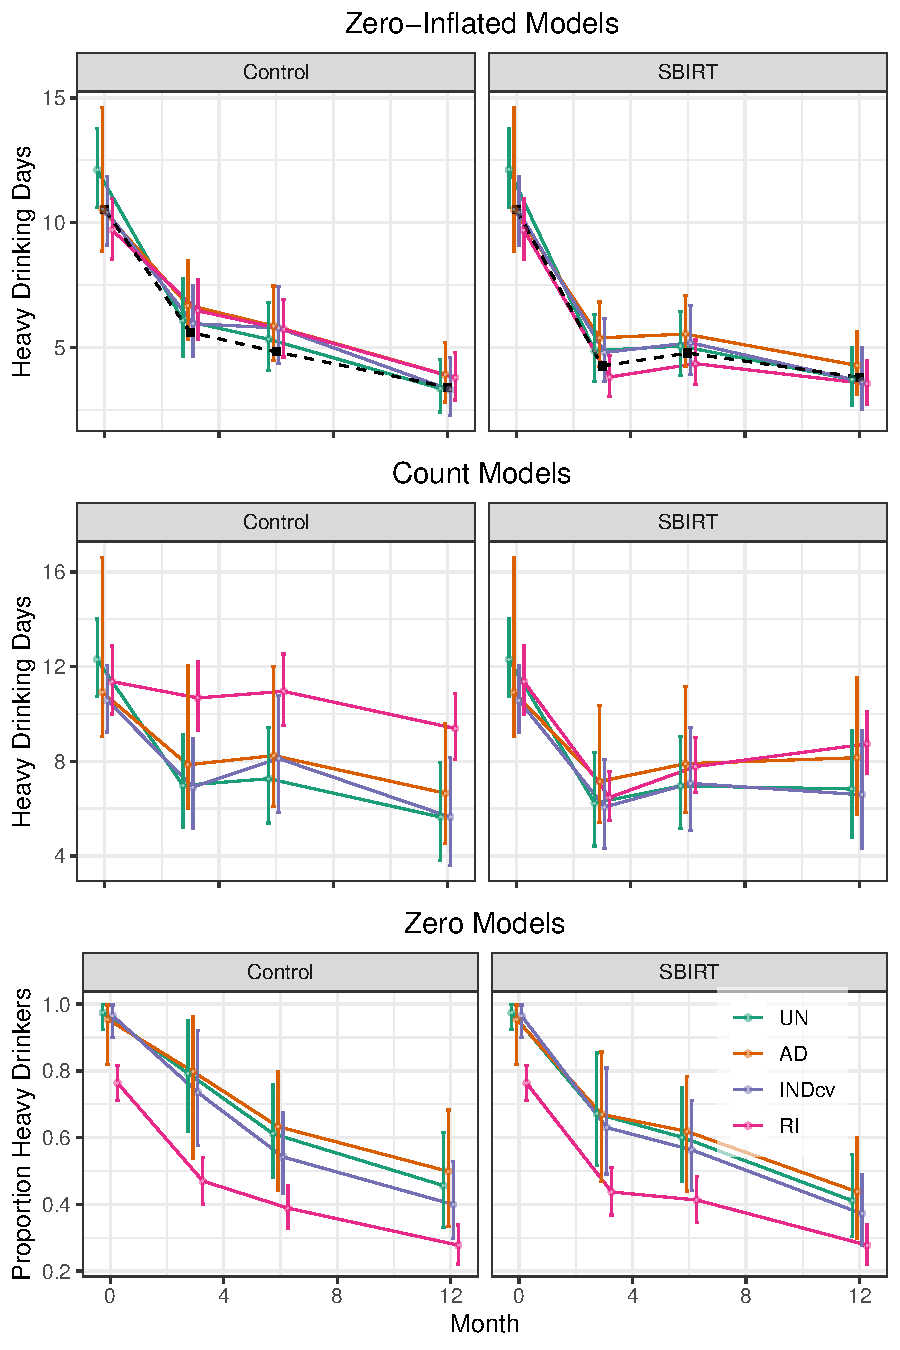
\includegraphics[scale = .8]{figures/mean_all_plot.pdf}
	\caption{Posterior means and 95\% CrIs for the three best fitting LOZIB models (UN, AD and INDcv) as well as the RI model for comparison. Plots on the left show the posterior means and CrIs for the control group and plots on the right show the same for the SBIRT group.  The top row of plots show the posterior summaries for the full zero-inflated models, while the middle and bottom rows display the posterior summaries of the count and zero models. The observed sample means for each group and time point are shown in black with a dashed line in top plots.}
	\label{fig:meanplots}
\end{figure}


\paragraph{Difference of Differences}
Figure \ref{fig:DoDplots} gives difference of differences (DoD) for all seven ZIB models, as well as the DoDs estimated from both the zero and the count parts of the model. The ARcv LOZIB and the RI models are bolded in orange and blue respectively.

\begin{figure}[t]
	\centering
	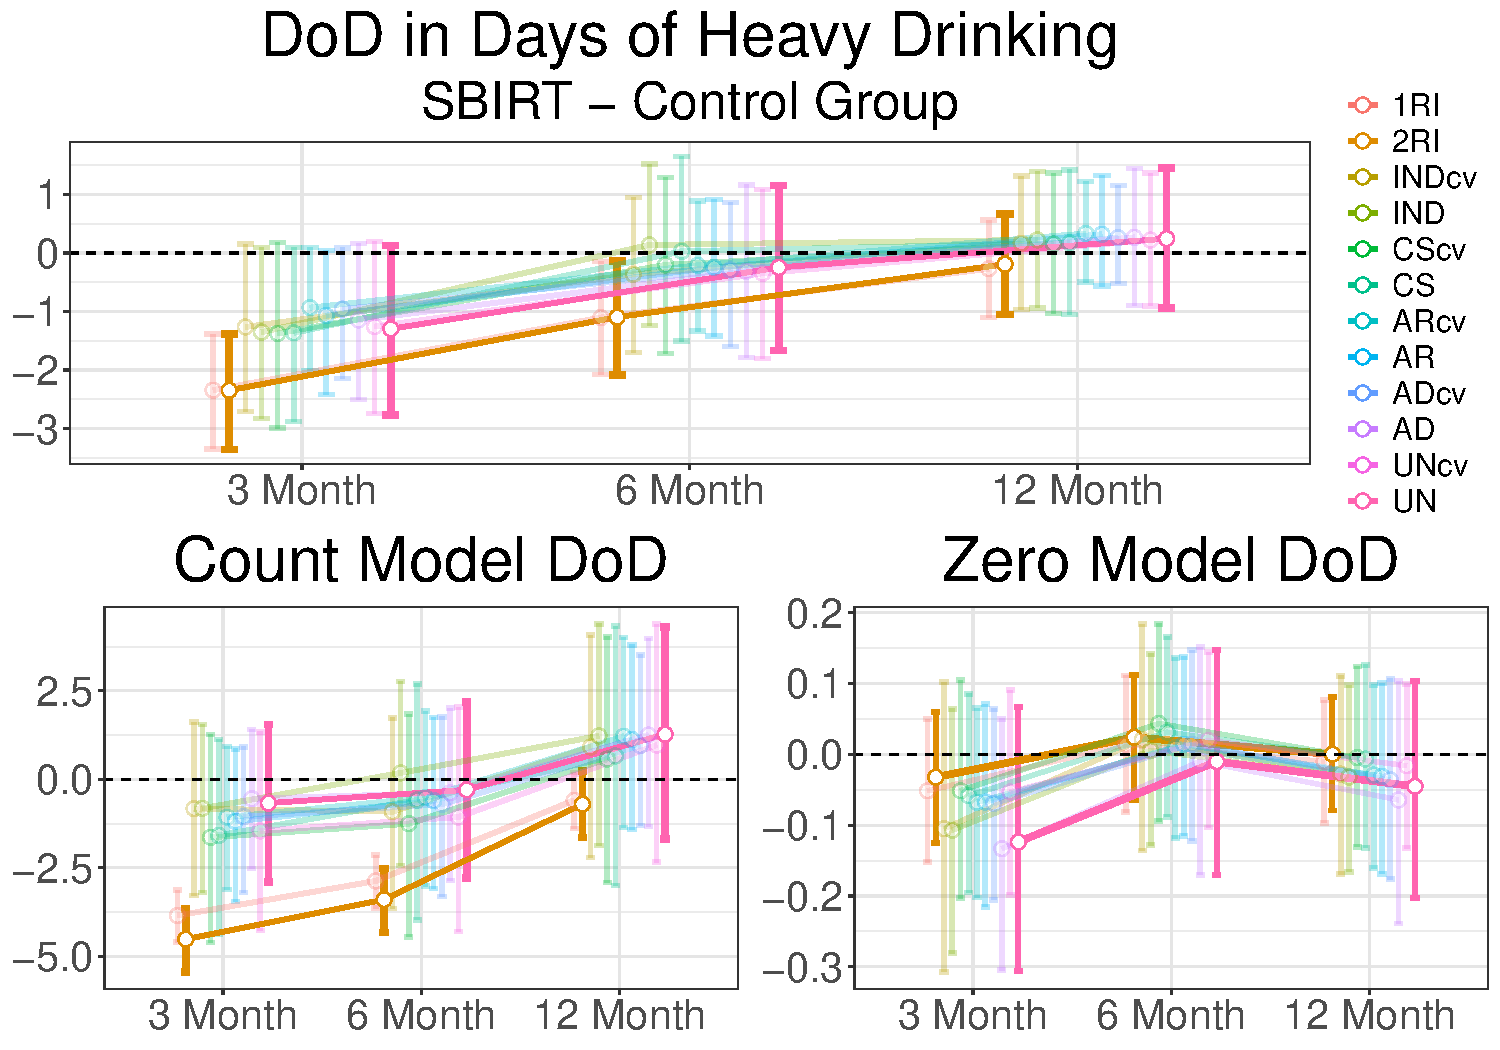
\includegraphics[scale=.5]{figures/DoDAllPlots.pdf}
	\caption{\textbf{Top:} Difference of differences (DoD) in mean days of heavy drinking measured as difference in change from baseline at each of the three follow up visits. Negative values indicate SBIRT group exhibited greater reductions in heavy drinking than control group. \textbf{Bottom left:} DoD in mean days of heavy drinking coming only from the count model, i.e., only among subjects who were deemed to be heavy drinkers. \textbf{Bottom right:} DoD in probability of being a heavy drinker coming from the zero model. Estimates and 95\% Bayesian credible intervals (CrI) are given for all seven ZIB models. The random intercept model (RI), given in blue, and the autoregressive constant variance model (ARcv), given in orange, are bolded for emphasis.}
	\label{fig:DoDplots}
\end{figure}


The RI model overestimates treatment effects compared to the better fitting LOZIB models (Figure \ref{fig:DoDplots}). At 3 and 6 month follow-up, the RI model 95\% Bayesian credible intervals for the DoDs do not include zero, a finding not shared by the six better fitting LOZIB models. In addition, the 3 month posterior means from each of the LOZIB models fall outside of the RI model credible intervals, further illustrating the disagreement between the LOZIB and RI models. Generally, the RI model estimates substantially stronger treatment effects than the LOZIB models .

There is relative consistency between the six LOZIB models. The estimates are not particularly sensitive to choices in covariance models, and thus modeling of overdispersion, rather than temporal correlation, may be the main driver of the improved performance of the LOZIB models. \bwr{Weiss comment: SHow us e's for AR and AD models first, before drawing this conclusion. I think we will likely find that there is some temporal correlation, it just doesn't have a large influence on LOO-IC.}

The lower left plot in Figure \ref{fig:DoDplots} gives the count model estimates for DoDs in days of heavy drinking out of the previous 90 among heavy drinkers. Again there is consistency among the six LOZIB models, while the RI model estimates greater reductions in drinking with much more narrow credible intervals.

The differences in treatment effects are minimal in the zero models (Figure \ref{fig:DoDplots}), which is not surprising as the zero models are parameterized identically across all seven ZIB models, and differences are only introduced through the connection to the count model. Zero model DoD estimates can be understood as the difference in the reduction in proportion of heavy drinkers between the two treatment groups. For example, the ARcv model estimates that at the 3 month follow-up, the reduction in proportion of heavy drinkers was .068 [\textit{95\%CrI}= (-.065, .202)] greater in the SBIRT group than in the control group.


%\begin{table}[t]
%	\centering
%	\resizebox{\textwidth}{!}{%
%		\begin{tabular}{rrllllll}
%			\hline
%			&&  \multicolumn{2}{c}{Observed} & \multicolumn{2}{c}{RI} & \multicolumn{2}{c}{INDcv}  \\ 
%			&& \multicolumn{1}{c}{Control} & \multicolumn{1}{c}{SBIRT} & \multicolumn{1}{c}{Control} & \multicolumn{1}{c}{SBIRT} & \multicolumn{1}{c}{Control} & \multicolumn{1}{c}{SBIRT}   \\
%			\hline
%			 \multirow[c]{4}{*}{Mean}& Baseline & \multicolumn{2}{c}{10.52} & \multicolumn{2}{c}{11.75 (10.42, 13.18)}  & \multicolumn{2}{c}{12.30 (10.87,  13.82)} \\ 
%			&3 Month & 5.60 & 4.25 & 8.01 (6.67, 9.45)& 5.00 (4.04, 6.07) & 5.57 (4.38, 6.94)& 5.57 (4.34, 6.98) \\ 
%			&6 Month  &  4.81& 4.77 & 7.14 (5.83, 8.54) & 5.61 (4.57, 6.75) & 6.21 (4.9, 7.70)& 4.84 (3.73, 6.11)\\ 
%			&12 Month   & 3.40 &3.79  & 4.92 (3.82, 6.12)& 4.64 (3.62, 5.77) & 3.65 (2.66, 4.85)& 4.51 (3.37, 5.86) \\ 
%			\hline
%	\end{tabular}}
%	\caption{Posterior means and 95\% Bayesian CrIs from RI and ARcv models. The top portion of the table gives mean days of heavy drinking out of the previous 90 days. The middle portion of the table gives DoD means and 95\% Bayesian CrIs, as well as the posterior probabilities that the DoD was less than zero - indicating a benefit of SBIRT over the control treatment. The bottom portion of the table gives posterior means and CrIs for the zero and count model random effects standard deviations ($\sigma_{1}$ and $\sigma_{2}$), the $\psi$ parameter, which models association between the count and zero models, and $\rho$, which is the within-individual across-time count model random effects correlation in the ARcv model. }
%	\label{tab:dodmean1}
%\end{table}


\begin{table}[t]
	\centering
	\resizebox{\textwidth}{!}{%
		\begin{tabular}{rrllll}
			\hline
			&& \multicolumn{2}{c}{RI} & \multicolumn{2}{c}{INDcv}  \\ 
			&& \multicolumn{1}{c}{Control} & \multicolumn{1}{c}{SBIRT} & \multicolumn{1}{c}{Control} & \multicolumn{1}{c}{SBIRT}  \\
			\hline
			\multirow[c]{4}{*}{Mean}&Baseline & \multicolumn{2}{c}{11.75 (10.42, 13.18)}  & \multicolumn{2}{c}{12.30 (10.87,  13.82)}  \\ 
			&3 Month & 8.01 (6.67, 9.45)& 5 (4.04, 6.07) & 5.57 (4.38, 6.94)& 5.57 (4.34, 6.98) \\ 
			&6 Month & 7.14 (5.83, 8.54) & 5.61 (4.57, 6.75) & 6.21 (4.9, 7.70)& 4.84 (3.73, 6.11)\\ 
			&12 Month & 4.92 (3.82, 6.12)& 4.64 (3.62, 5.77) & 3.65 (2.66, 4.85)& 4.51 (3.37, 5.86)\\ 
			\hline
			\multirow[c]{4}{*}{DoD}& &  \multicolumn{1}{c}{ DoD}&  \multicolumn{1}{c}{p(DoD $<$ 0)} &  \multicolumn{1}{c}{DoD} &    \multicolumn{1}{c}{p(DoD $<$ 0)}\\
			&3 Month& \multicolumn{1}{c}{-2.35 (-3.36, -1.38)} & \multicolumn{1}{c}{1} & \multicolumn{1}{c}{ -0.934 (-2.01, .963)} & \multicolumn{1}{c}{.963}\\ 
			&6 Month& \multicolumn{1}{c}{ -1.10  (-2.08, -.134)} & \multicolumn{1}{c}{.987} & \multicolumn{1}{c}{ -.211 (-1.33 , .646)} & \multicolumn{1}{c}{.646}\\ 
			&12 Month & \multicolumn{1}{c}{ -.193 (-1.05, .666)} & \multicolumn{1}{c}{.674 }& \multicolumn{1}{c}{.331 (-.500 , .217)} & \multicolumn{1}{c}{.217}\\ 
			\hline
			Zero RE SD & $\sigma_{1}$ & \multicolumn{2}{c}{1.7 (1.39, 2.02)}& \multicolumn{2}{c}{1.8 (1.32, 2.31)}\\ 
			Count RE SD  & $\sigma_{2} $ & \multicolumn{2}{c}{1.98 (1.78, 2.2)}& \multicolumn{2}{c}{1.82 (1.68, 1.98)}\\ 
			&$\psi$ & \multicolumn{2}{c}{.744 (.308, 1.15)} & \multicolumn{2}{c}{.826 (.249, 1.41)} \\ 
			&$\rho$ & \multicolumn{2}{c}{ -}& \multicolumn{2}{c}{.732 (.647, .797)} \\ 
			\hline
	\end{tabular}}
	\caption{Posterior means and 95\% Bayesian CrIs from RI and ARcv models. The top portion of the table gives mean days of heavy drinking out of the previous 90 days. The middle portion of the table gives DoD means and 95\% Bayesian CrIs, as well as the posterior probabilities that the DoD was less than zero - indicating a benefit of SBIRT over the control treatment. The bottom portion of the table gives posterior means and CrIs for the zero and count model random effects standard deviations ($\sigma_{1}$ and $\sigma_{2}$), the $\psi$ parameter, which models association between the count and zero models, and $\rho$, which is the within-individual across-time count model random effects correlation in the ARcv model. }
	\label{tab:dodmean}
\end{table}
\bwr{Weiss: Factors of 50 \% to 100\% different between RI and ARcv. How does raw data compare?}


%\begin{table}[ht]
%	\caption{UN model mean estimates and 95\% Bayesian CrI from zero and count models for each treatment group at each time point for SBIRT data.  Zero model estimates are proportion of subjects that engage in heavy alcohol use, count model estimates are the expected number of days per 90 of heavy alcohol use among users. Middle portion gives mean DoD estimates for each part of the hurdle model at each time point as well as the average across all follow-up time points (All F-U).  $\psi$ is the parameter modeling the dependency between zero and count models.}
%	\centering
%	\resizebox{\textwidth}{!}{%
%		\begin{tabular}{rrllll}
%			\hline
%			&& \multicolumn{2}{c}{RI} & \multicolumn{2}{c}{ARcv}  \\ 
%			&& \multicolumn{1}{c}{Control} & \multicolumn{1}{c}{SBIRT} & \multicolumn{1}{c}{Control} & \multicolumn{1}{c}{SBIRT}  \\
%			\hline
%			Mean&Baseline & \multicolumn{2}{c}{ 9.61(8.39, 10.9)}  & \multicolumn{2}{c}{6.85 (5.44, 8.45)}  \\ 
%			&3 Month & 5.62 (4.57, 6.79) & 3.27 (2.58, 4.08) & 3.25 (2.36, 4.34)& 2.32 (1.62, 3.19) \\ 
%			&6 Month & 4.77 (3.81, 5.85) & 3.68 (2.89, 4.57) & 2.45 (1.66, 3.44)& 2.24 (1.50, 3.15)\\ 
%			&12 Month & 2.96 (2.25, 3.78) & 2.77 (2.08, 3.57) & 1.24 (.751, 1.9)& 1.57 (.958, 2.38) \\ 
%			\hline
%			DoD & & &  \multicolumn{1}{c}{p(DoD $<$ 0)} &&    \multicolumn{1}{c}{p(DoD $<$ 0)}\\
%			&3 Month& \multicolumn{2}{c}{-2.35 (-3.36, -1.38)}  & \multicolumn{2}{c}{ -0.934 (-2.01, .963)}  \\ 
%			&6 Month& \multicolumn{2}{c}{ -1.10  (-2.08, -.134)}  & \multicolumn{2}{c}{ -.211 (-1.33 , .646)}  \\ 
%			&12 Month & \multicolumn{2}{c}{ -.193 (-1.05, .666)}  & \multicolumn{2}{c}{.331 (-.500 , .217)}  \\ 
%			\hline
%			&$\rho$ & && \multicolumn{2}{c}{.04 (.003, .09)} \\ 
%			&$\psi$ & && \multicolumn{2}{c}{.04 (.003, .09)} \\ 
%			\hline
%	\end{tabular}}
%\end{table}





%\begin{figure}[t]
%	\centering
%	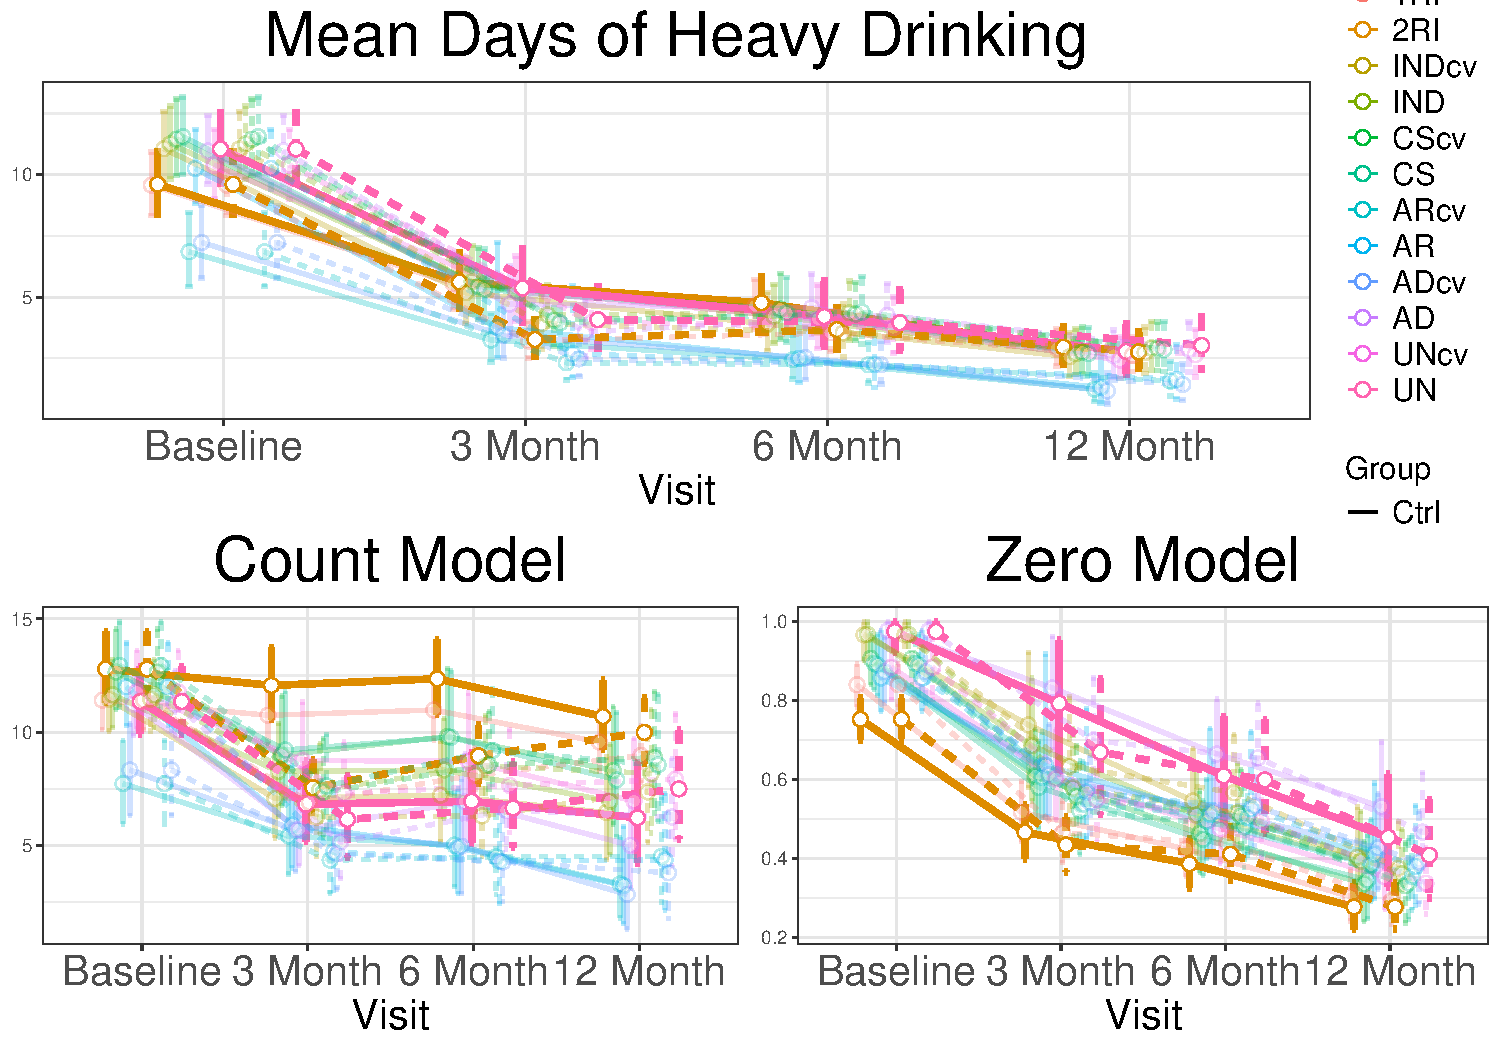
\includegraphics[scale=.5]{figures/MeanAllPlots.pdf}
%	\caption{\textbf{Top:} Posterior means and 95\% CrIs for mean days of heavy drinking per 90 days for each of the 7 fitted models for both SBIRT (Trt) and control (Ctrl) groups. Both treatment groups are estimated to have reductions in days of heavy drinking according to all models. \textbf{Bottom left:} Mean days of heavy drinking coming only from the count model, that is, only among subjects who were deemed to be heavy drinkers. \textbf{Bottom right:} Posterior means and 95\% CrIs for probability of being a heavy drinker at each visit for both treatment groups. In all plots, the random intercept model (RI), given in blue, and the autoregressive constant variance model (ARcv), given in orange, are bolded for emphasis.}
%	\label{fig:meanplots}
%\end{figure}


\bwr{Weiss Notes: Rather large range among models in the zero model estimates. }

\section{Discussion}

We developed a class of longitudinal overdispersed zero-inflated binomial (LOZIB) models which extend previous models through the inclusion of observation-level random effects (OLRE) in the count model regression. These OLRE provide increased flexibility to account for both overdispersion and correlation over time. We demonstrated LOZIB models with six different covariance models, which we applied to the SBIRT data to model counts of days of heavy drinking out of the previous 90 days. The LOZIB models showed improved ability to fit the data over a RI ZIB model, however differences between the 6 LOZIB models were small. In addition to improving fit, the LOZIB models yielded different inference than the RI model. These differences could be impactful, for example, if policy makers were to use 95\% Bayesian credible intervals to gauge significance of a treatment effect, the SBIRT intervention would be found to be effective at 3 and 6 months under the RI model, but not under the better fitting LOZIB models. 

We hypothesize that the superiority of the LOZIB models in the SBIRT analysis stem mainly from the LOZIB models ability to handle excess variation. Failure to adequately account for overdispersion in count models can lead to bias both mean and variance estimates. In the SBIRT analysis, the general use of a LOZIB model is an important improvement, though the choice of which covariance model to use within the LOZIB model is not particularly influential. In larger data sets with more time points, differences in covariance models may be more noticeable. The random effects covariance matrix grows quickly with the number of time points, as does the difference in number of parameters to estimate between, for example, the ARcv (2 parameters), and the UN models ($\frac{n (n-1)}{2}$ parameters).  

We also attempted to fit the SBIRT data with frequentist RI models using the glmmTMB R package \citep{brooks2017glmmtmb}, but the models failed to converge on reliable model estimates. To our knowledge, it is not possible to fit LOZIB type models using the package. In contrast, under a Bayesian framework, it is straightforward to fit both the RI ZIB and LOZIB models using Stan software \citep{gelman2015stan}, and all models converged yielding valid inference. In addition, the SBIRT analysis illustrates the usefulness of Bayesian methods to construct valid credible intervals for functions of model parameters. Using our methods, it was straightforward to produce estimates and intervals for mean days of heavy drinking as well as difference of differences and probability of a treatment effect (Table \ref{tab:dodmean}).

There are a number of possible extensions of the LOZIB models presented in this paper. The LOZIB models we developed were designed for nominal time, such as in the SBIRT study where observations were measured at pre-specified times. In other settings one may wish to adapt LOZIB models to handle continuously measured time. This change would be reflected both in the random effects specification as well as the regression parameterization where one may estimate a continuous time effect. Additionally, the LOZIB models may be adapted to model multivariate outcomes where one may specify, for example, a vector autoregressive model to account for correlation both over time and between different outcomes.

Overdispersed longitudinal zero-inflated data can occur in many settings beyond substance use, and for these situations we recommend LOZIB models to researchers due to their ability to account for excess variation and longitudinal correlation. Failure to properly account for these two aspects of data can give rise to misleading inference as we saw in the case of the SBIRT study. Overall, we present LOZIB models as an important improvement over previous methods for overdsipersed longitudinal zero-inflated data.


\newpage

\section{References}

\bibliography{lozib}

\end{document}
